\begin{frame}
 \frametitle{Cross Product}

\begin{center}
 (\textbf{vector}, \textbf{vector}) $\to$ \textbf{vector}
\end{center}

\begin{figure}[h]
  \psfrag{u}{$\textbf{u}$}
  \psfrag{v}{$\textbf{v}$}
  \psfrag{ovu}{$\textbf{orth}_{\bm{u}} \textbf{v}$}
  \psfrag{a}{$\alpha$}
  \psfrag{uxv}{$\textbf{u} \times \textbf{v}$}
  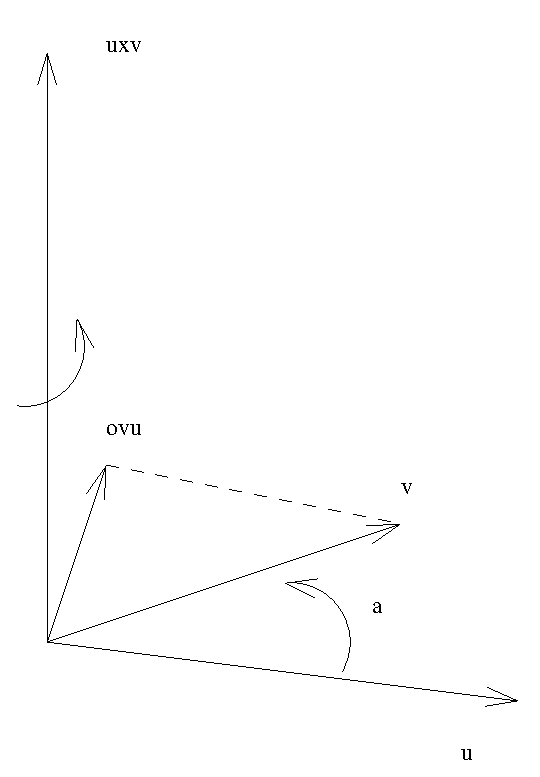
\includegraphics[height=1in]{../../modules/vectors/pictures/ok-cross_product.eps}
\end{figure}

\begin{itemize}
 \item If $\textbf{u}$, $\textbf{v}$ are non-zero and non-collinear vectors:\\
\begin{center}
 $\textbf{u} \times \textbf{v}$ is the vector determined by:
\end{center}
%
\begin{itemize}
 \item Support of direction of $\textbf{u} \times \textbf{v}$:
perpendicular to both $\textbf{u}$ and $\textbf{v}$;
 \item Direction of $\textbf{u} \times \textbf{v}$: given by Right Hand Rule;
 \item Magnitude of $\textbf{u} \times \textbf{v}$: product of $|\textbf{u}|$ and $|\textbf{orth}_{\bm{u}} \textbf{v}|$
%
$$|\textbf{u} \times \textbf{v}| = |\textbf{u}| \, |\textbf{orth}_u \textbf{v}| = |\textbf{u}| |\textbf{v}| \sin{\alpha}$$
%
\end{itemize}
\item If $\textbf{u}=\textbf{0}$ or $\textbf{v}=\textbf{0}$ or
$\textbf{u}$ and $\textbf{v}$ are collinear: \pause $\textbf{u} \times \textbf{v} = \textbf{0} $.
%
\end{itemize}

\end{frame}